\section{Overlapping Reconstructions}
\label{sec:overlapping}

\subsection{Purpose}

Frazier et al. demonstrate that the sona of a given interrogation pulse is significantly longer than the pulse that generated it~\cite{nltr-wave-chaotic}. This stands to reason, given that the sona represents reflections of the initial pulse shifted in time by differing path lengths.

To start with, an important feature of this method is spatial fidelity: the ability to deliver highly localized reconstruction to a reciever. In the interest of delivering more energy with each packet, there is a desire to make the duration of the reconstruction longer. To do this, however, would reduce the bandwidth of the interrogation pulse and reconstruction. The bandwidth of the interrogation pulse translates to the number of eigenmodes available for comunication between the transmitter and reciever. The requirement for a suitibly large bandwidth restricts the duration or temporal localization of the interrogation pulse and reconstruction. As a result, increasing the energy delivered per reconstruction packet by extending the duration of the interrogation pulse is not a favorable option as it reduces the spatial fidelity of the reconstruction.

To increase the amount of energy transmitted, we propose two modifications to the time reversal scheme. Either the amount of energy contained within each packet can be inflated, or the frequency of packets can be increased. Increasing the size of the reconstruction is a trivial matter; by amplifying the time reversed sona before reinjection, the reconstruction is correspondingly amplified. We desire to send reconstructions more frequently than the length of the sona will allow. However, transmitting multiple sonas at once from the same antenna is possible--copying and shifting the signal in time can allow several signals to be sent in less time than the sum of the individual sona time lengths. This will in turn result in multiple transmitted reconstructions, and improved power transmission.

A concern with the above method is whether or not it would result in lost information and consequently degraded reconstruction quality. Sonas are sinusoidal signals--if overlaid, they will interfere constructively and destructively. Destructive interference may result in the ``deletion'' of transmission paths, reducing the efficiency of the TR process and decreasing the fidelity of the created reconstructions. In this experiment, we are interested in understanding the degree to which superimposing sonas will degrade the ability to transmit energy between ports using linear time reversal.

\subsection{Methodology}

This test sought to evaluate the practicality of overlapping sonas as a method of transmitting power. This experiment was done using the basic, two-port linear time reversal scheme, first described in Section~\ref{sec:ltr-meth}. A diagram of this scheme appears as ~\fig{ltr-process}.

\begin{figure}[h!]
\centering
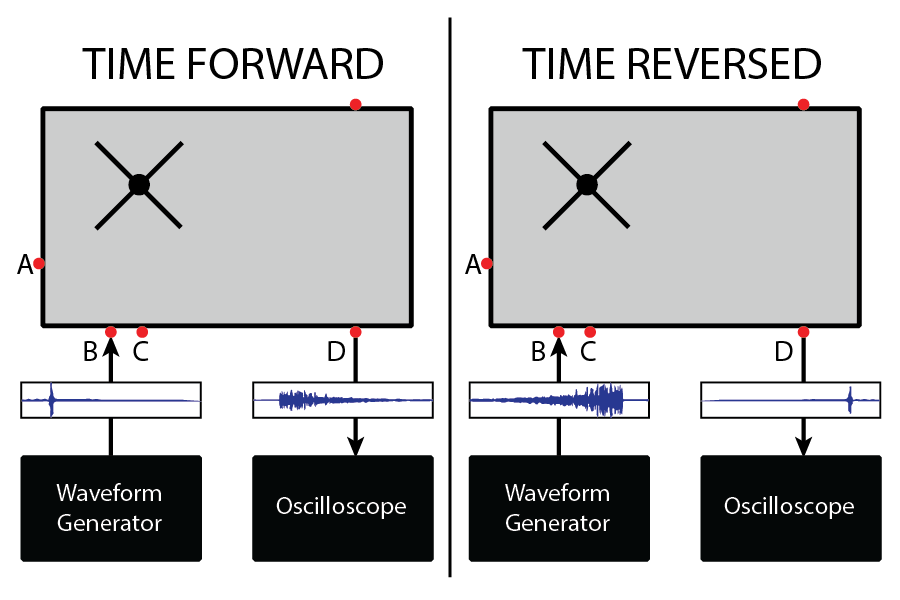
\includegraphics[width=0.85\textwidth]{linear/ltr-process}
    \caption[Experimental Setup]{A diagram of our typical two-port linear time reversal scheme. In the time forward step, a pulse is broadcast from antenna port B and a sona collected at D. In the time reversed step, the reversed sona is broadcast from B and a reconstruction occurs at D. This setup takes advantage of spatial as well as temporal reciprocity to avoid having to record and broadcast from the same port, which greatly complicates cabling and introduces losses from the switches.}
    \label{fig:ltr-process}
\end{figure}

A sona was generated with a 3.9 GHz interrogation pulse. To verify that the sona could converge on the target, it was time reversed without any further manipulation, and injected back into the cavity. The reconstruction was recorded and compared to the original interrogation pulse to check for irregularities.

Once the efficacy of the single sona was established, the experiment was modified. Several sonas were superimposed with a constant time shift, resulting in evenly spaced copies of the verified sona across the total broadcast window. Figure~\ref{fig:overlapping-sonas} gives an example of sonas overlapping in this way. The resulting signal was then time reversed and broadcast through the linear system in the same manner as before, which resulted in the reconstructions in Figure~\ref{fig:overlapping-recons}. This test was repeated many times, with the number of sonas superimposed within the 15~$\mu$s broadcast window varying from one to three hundred. This corresponds to repetition rates between 66 kHz and 20 MHz.

\begin{figure}
\centering
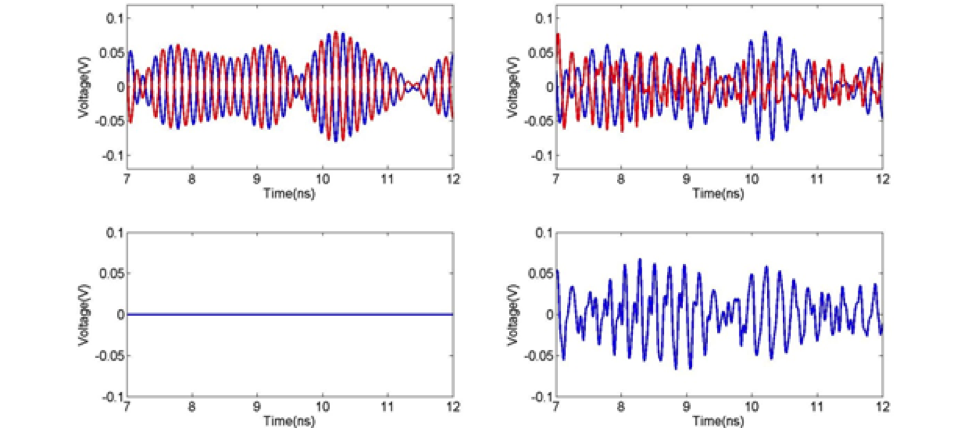
\includegraphics[width=0.85\textwidth]{overlapping/sonas}
\caption[Overlapped sonas]{Overlapped sonas with a spacing of 7.5~$\mu$s.}
\label{fig:overlapping-sonas}

\vspace*{\floatsep}% http://tex.stackexchange.com/q/26521/5764

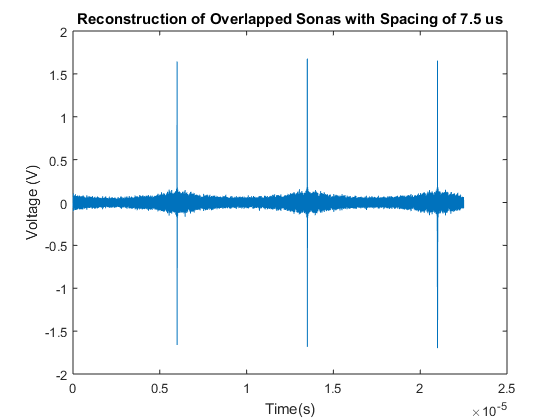
\includegraphics[width=0.85\textwidth]{overlapping/recons}
\caption[Overlapped reconstructions]{Reconstructions resulting from the sonas in~\ref{fig:overlapping-sonas}.}
\label{fig:overlapping-recons}
\end{figure}


\subsection{Results}

Increasing the number of sonas should increase the amount of power transmitted in a given time frame, if the amplitude of each reconstruction remains constant. We hypothesized that overlapping reconstructions by linearly superimposing sonas would not decrease the size of the reconstructions. As a result, a great amount of effective power was transmitted per duty cycle. Our experiments seemed to support this conjecture, in that the number of reconstructions in the cycle could be increased while maintaining their characteristic shape. However, the size of the packets did decrease as the number of reconstructions within the window became larger.

We believe these results to be a combination of two factors. The loss of information due to destructive interference during sona superposition, and the function of power scaling within the PSG signal generator both may have contributed to this decreasing trend. The generator attempts to level a preset amount of power across the entire broadcast window, which is split among the multiple reconstructions.
To better model how these reconstructions would interact with a practical WPT system, we also examined the ``total \ptp{} voltage,'' which we defined as the maximum \ptp{} voltage multiplied by the number of reconstructions present within the measurement window. This quantity emulates the energy that would be rectified within the same time window, so we can compare the various repetition rates with regard to the energy that a receiver would accept within that time frame. This correlation is plotted in Figure~\ref{fig:overlapping-total-voltage}.

Important to note is the overall increasing trend, which resembles a square root function. This is expected, as the power is expected to vary linearly with the number of overlaid sonas, and is proportional to the \ptp{} voltage squared. The positive correlation between repetition rate and total voltage indicates that the use of this technique would be very valuable for a WPT scheme. We can acquire a sona and then broadcast the time reversed version at very high repetition rates to transmit large amounts of energy to the receiver. Coupled with an arbitrary amplification according to the application's needs, this modification to a time reversal WPT system shows promise for increasing the quantity of power that can be transferred.

\begin{figure}
\centering
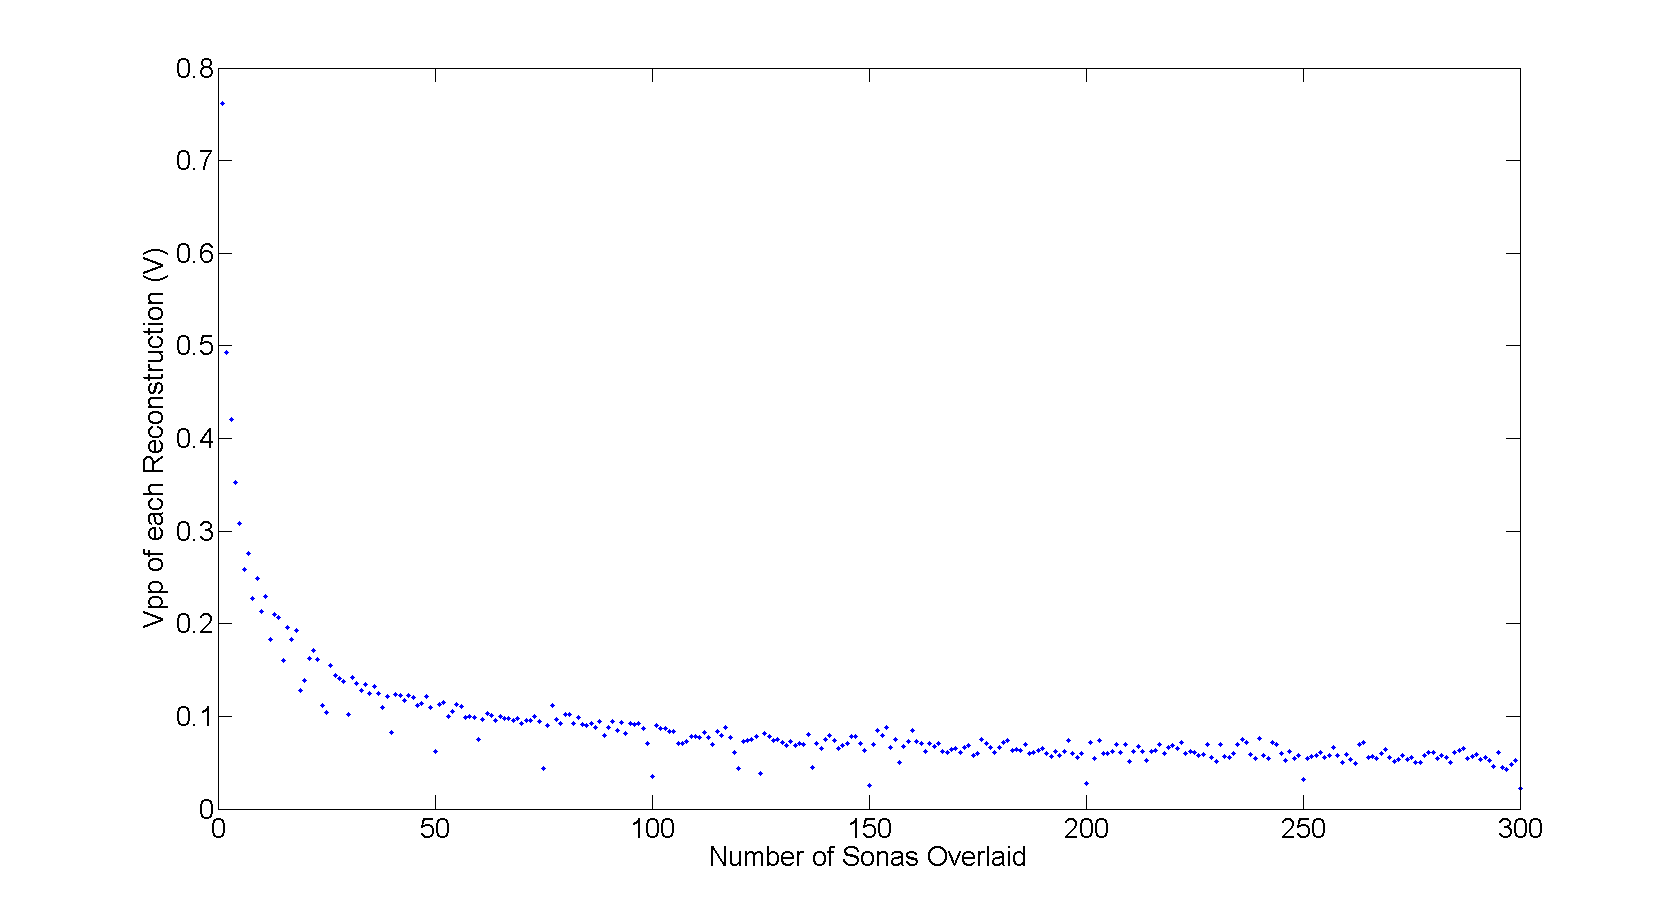
\includegraphics[width=0.85\textwidth]{overlapping/voltage_per_recon}
\caption[Max \ptp{} voltage from overlapped reconstructions]{Max \ptp{} voltage versus number of overlapped reconstructions.}
\label{fig:overlapping-vpp}

\vspace*{\floatsep}% http://tex.stackexchange.com/q/26521/5764

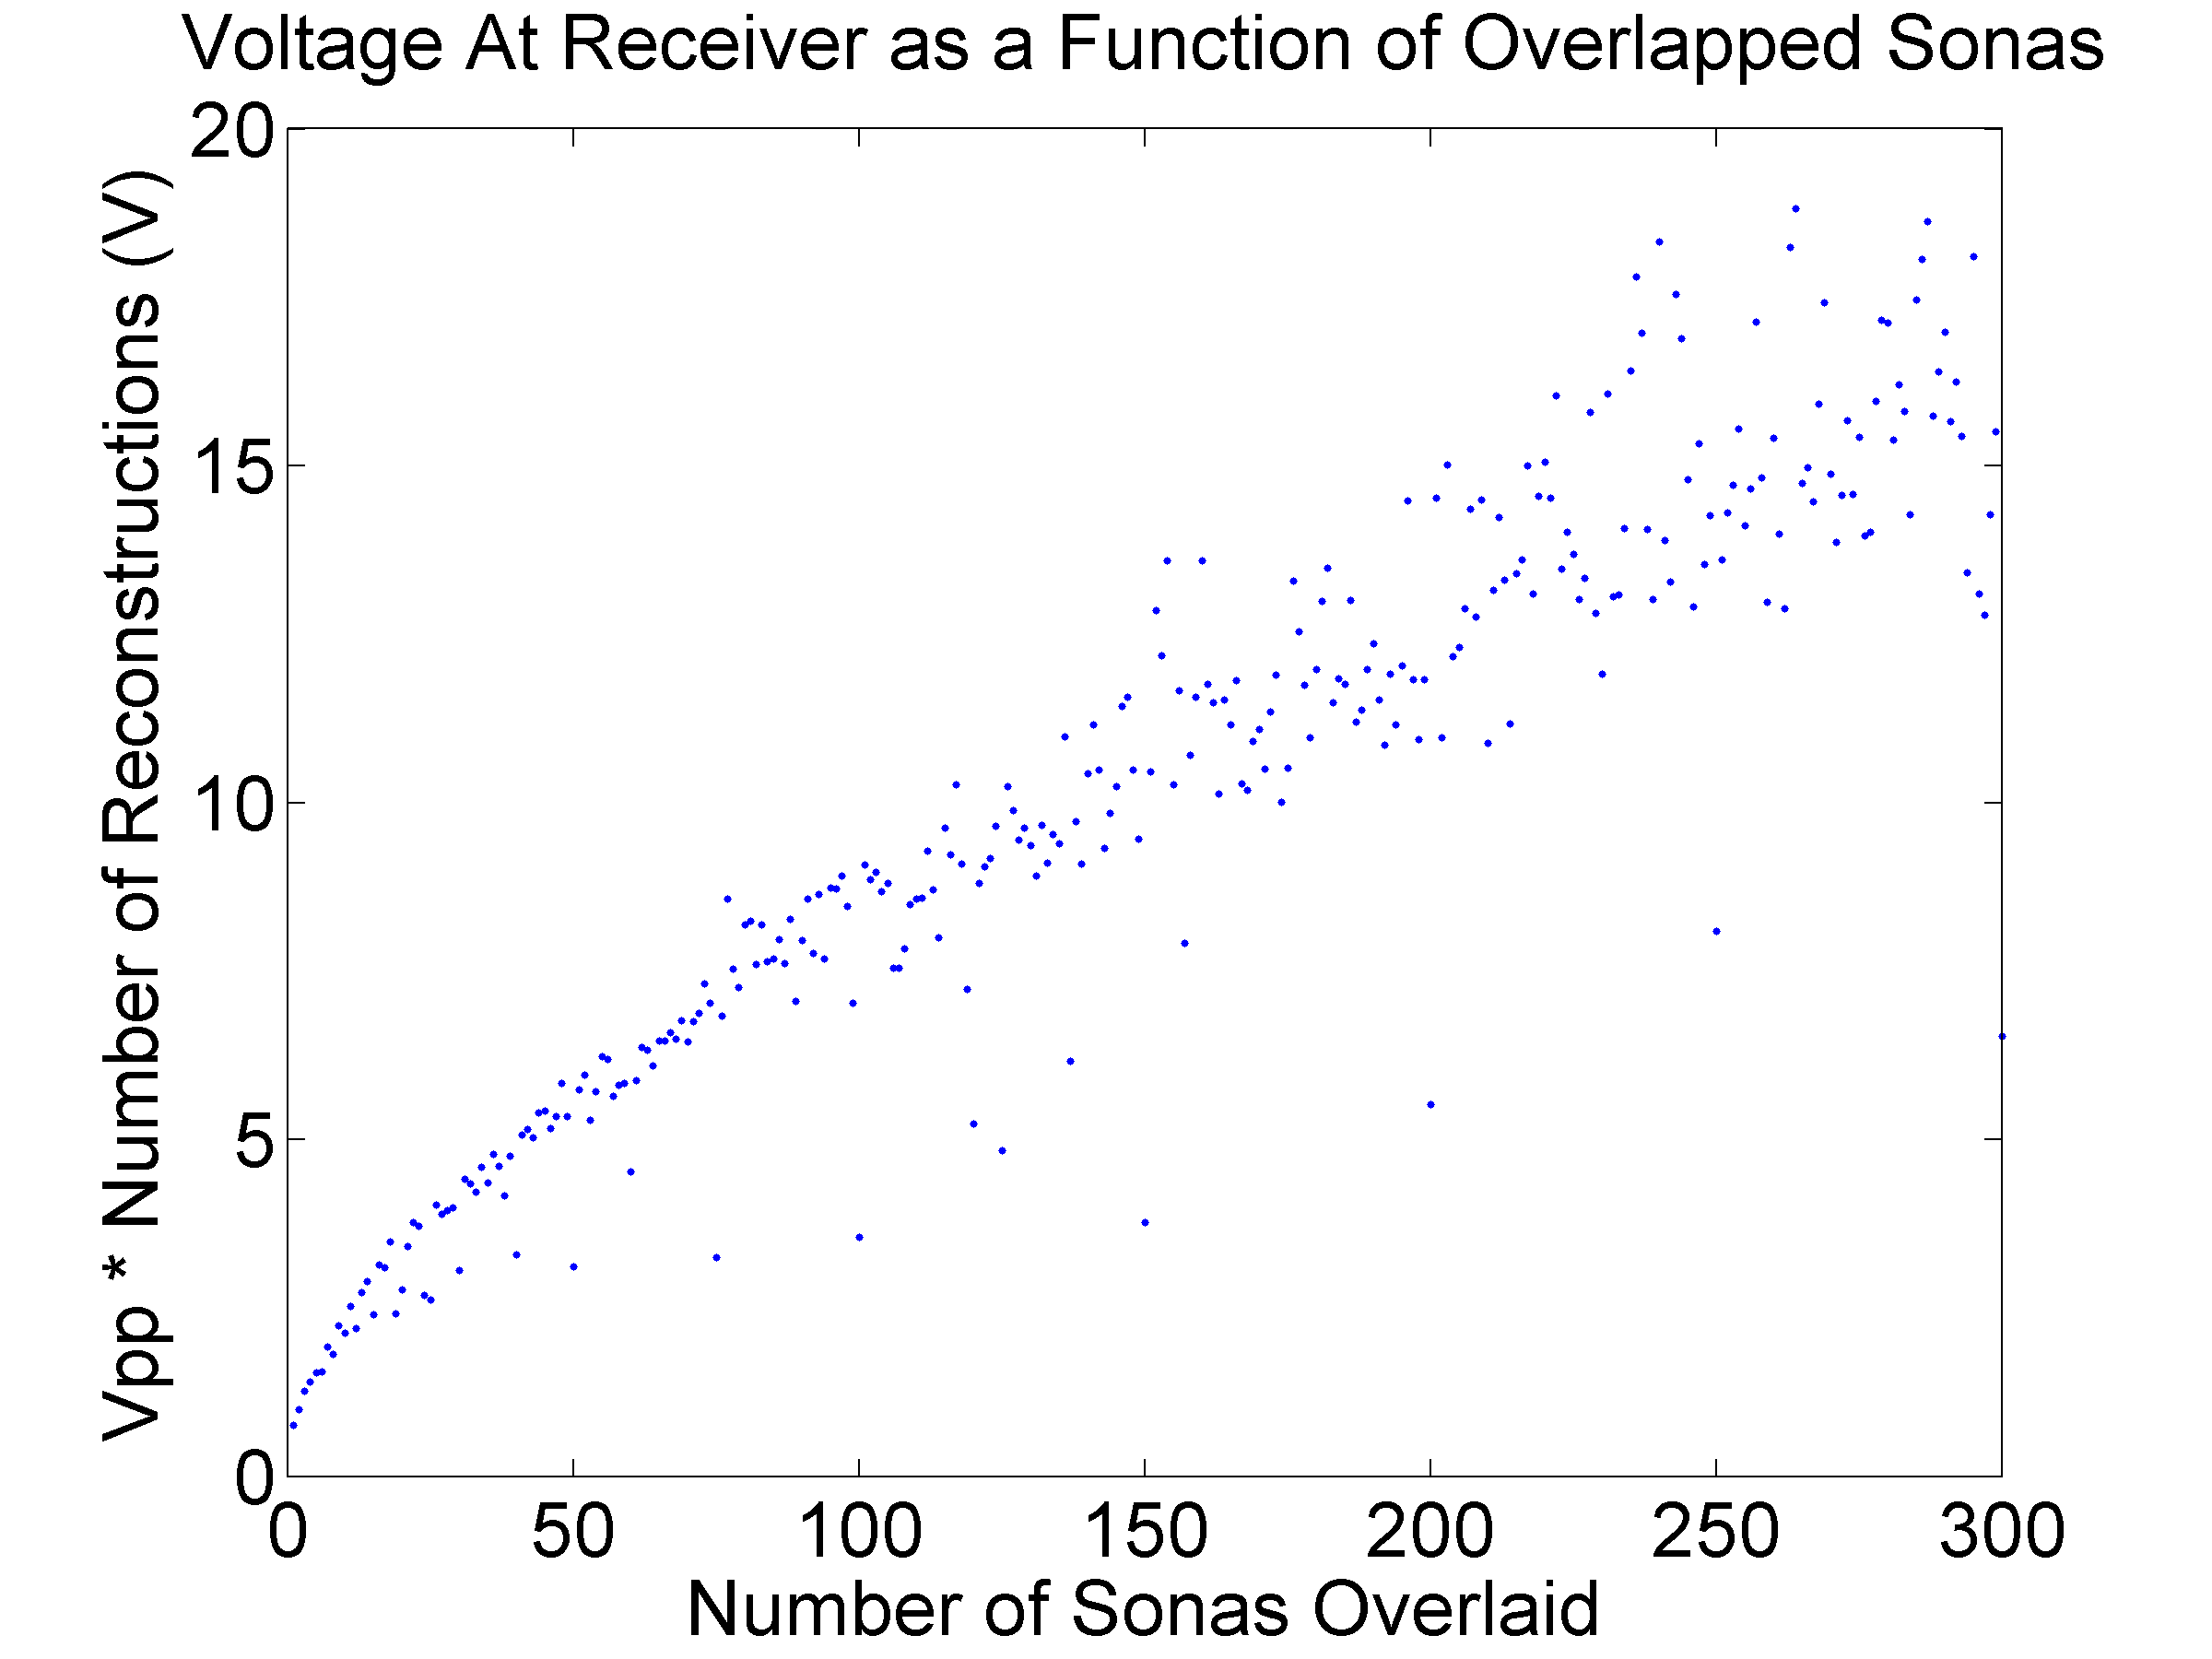
\includegraphics[width=0.85\textwidth]{overlapping/total_voltage}
\caption[Total \ptp{} voltage from overlapped reconstructions]{Total \ptp{} voltage versus number of overlapped reconstructions.}
\label{fig:overlapping-total-voltage}
\end{figure}
